% 图 17.3 —— 由 `checks/emit_hand.py` 自动拼出（probe 精测 + prims2 图元分解）
%%
% ⚠ 这是**稿子不是成品**：跑 `checks/checkhand.py 17.3` 看指标 + 看叠合图。
%%
%% ⚠ 待核：
%   · 本图 probe 报出阴影族 1 个 —— **本脚本不生成阴影**（要照原书手写）；prims2 的 strokes 里可能含阴影线，核对时留意别画重
%   · 可疑字形 1 项（空心圈 ⊙ 常被认成字母 o）—— 见文件末
%%
\documentclass[12pt]{standalone}
\usepackage{fontspec}
\setsansfont{Arial}
\newfontfamily\mfallback{DejaVu Sans}
\usepackage{tikz}
\begin{document}
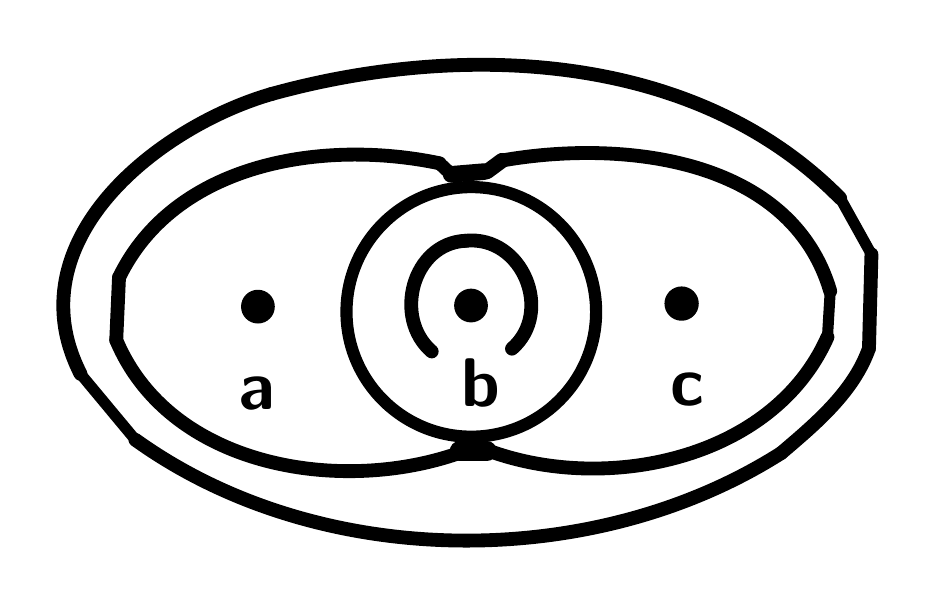
\begin{tikzpicture}[x=1pt, y=-1pt, line width=4.4pt, line cap=round, line join=round]

  %% ════ 填充区（prims2 的 fills）════

  %% ════ 直线段（prims2 的 strokes）════
  \draw[line width=5.0pt] (32.0,112.9) -- (33.0,90.3);
  \draw[line width=4.8pt] (148.8,49.0) -- (152.0,52.0);
  \draw[line width=6.0pt] (165.0,52.0) -- (153.0,53.0);
  \draw[line width=7.0pt] (156.0,153.0) -- (166.0,153.0);
  \draw[line width=4.0pt] (289.0,111.8) -- (290.0,95.2);
  \draw[line width=5.5pt] (171.4,48.0) -- (166.0,52.0);
  \draw[line width=4.0pt] (293.6,61.6) -- (304.9,81.9);
  \draw[line width=5.0pt] (304.9,81.9) -- (304.0,115.9);
  \draw[line width=4.0pt] (38.9,148.9) -- (19.1,125.1);

  %% ════ 曲线（prims2 的 curves —— 三段式，坐标同为 (y,x)）════
  \draw[line width=5.0pt] (155.0,154.0) .. controls (112.6,168.5) and (51.4,158.9) .. (32.0,112.9);
  \draw[line width=5.0pt] (33.0,90.3) .. controls (53.2,48.6) and (106.9,40.2) .. (148.8,49.0);
  \draw[line width=5.0pt] (167.0,153.0) .. controls (209.1,168.3) and (269.3,156.2) .. (289.0,111.8);
  \draw[line width=5.0pt] (290.0,95.2) .. controls (275.7,46.6) and (214.3,40.4) .. (171.4,48.0);
  \draw[line width=5.0pt] (175.0,116.0) .. controls (190.2,102.8) and (178.8,74.9) .. (158.2,77.0);
  \draw[line width=5.0pt] (158.2,77.0) .. controls (139.0,77.9) and (131.9,104.9) .. (146.0,117.0);
  \draw[line width=5.0pt] (88.0,24.0) .. controls (156.1,5.1) and (240.9,8.0) .. (293.6,61.6);
  \draw[line width=5.0pt] (304.0,115.9) .. controls (298.5,131.5) and (285.0,142.9) .. (272.3,153.7);
  \draw[line width=5.0pt] (272.3,153.7) .. controls (204.4,196.9) and (105.0,196.4) .. (38.9,148.9);
  \draw[line width=5.0pt] (19.1,125.1) .. controls (-5.3,77.2) and (47.0,35.9) .. (88.0,24.0);

  %% ════ 圆 / 椭圆（probe 精测）════
  \draw (160.3,102.7) circle (45.1);

  %% ════ 实心点 ════
  \fill (236.3,99.7) circle (6.2);
  \fill (160.2,100.4) circle (6.1);
  \fill (83.2,100.8) circle (6.1);

  %% ════ 标签（probe 直接给的 \node 行）════
  %% ⚠ 全部补了 fill=white：文字在最上层，否则与曲线交叉干扰
     \node[anchor=center,inner sep=0pt,fill=white,font=\fontsize{30.0}{37.5}\selectfont] at (163.8,128.2) {\textsf{\textbf{\textit{b}}}};   % box(154,116,17,22)
     \node[anchor=center,inner sep=0pt,fill=white,font=\fontsize{30.5}{38.1}\selectfont] at (238.3,131.0) {\textsf{\textbf{\textit{c}}}};   % box(230,121,15,17)
     \node[anchor=center,inner sep=0pt,fill=white,font=\fontsize{32.0}{40.0}\selectfont] at (83.1,132.1) {\textsf{\textbf{\textit{a}}}};   % box(74,122,16,17)

  % 钉死画布：否则超出的图元/控制点会把页面撑大，1:1 回比就失准
  \pgfresetboundingbox
  \path[use as bounding box] (0,0) rectangle (316,195);
\end{tikzpicture}
\end{document}

% ⚠ 待核清单（probe 拿不准，人眼过一遍）：
%   · 未识别/跳过：⑤ 跳过/未识别的字形
